\documentclass[a4paper]{jarticle}

\usepackage{moreverb}
\usepackage{ascmac}
\usepackage{amsmath}
\usepackage{enumerate}
\usepackage{eclbkbox}
\usepackage[dvipdfmx]{graphicx}
\usepackage{comment}

\setlength{\textheight}{\paperheight}   % 紙面縦幅を本文領域にする(BOTTOM=-TOP)
\setlength{\topmargin}{4.6truemm}       % 上の余白を30mm(=1inch+4.6mm)に
\addtolength{\topmargin}{-\headheight}  % 
\addtolength{\topmargin}{-\headsep}     % ヘッダの分だけ本文領域を移動させる
\addtolength{\textheight}{-60truemm}    % 下の余白も30mm(BOTTOM=-TOPだから+TOP+30mm)

\setlength{\textwidth}{\paperwidth}     % 紙面横幅を本文領域にする(RIGHT=-LEFT)
\setlength{\oddsidemargin}{-0.4truemm}  % 左の余白を25mm(=1inch-0.4mm)に
\setlength{\evensidemargin}{-0.4truemm} % 
\addtolength{\textwidth}{-50truemm}     % 右の余白も25mm(RIGHT=-LEFT)

\begin{document}
\title{センシング工学特論\\レポート課題【課題 II 】}
\author{3G150131 松井 健人}
\date{2015年6月17日}
\maketitle

%-----------------------------
%1章
%-----------------------------

\section{課題 I }
\textbf{観測方程式}
\begin{equation}
z = x_0 + {x_1}a + {x_2}{a^2} = 
\left[  \ 1\ \ a\ \ a^2\   \right]
 \begin{bmatrix}
{x_0} \\ {x_1} \\{x_2} \\ 
\end{bmatrix}   + w= 
\mbox{\boldmath $a$}^{T}\mbox{\boldmath $x$} + w
\end{equation}
に関して下表の観測値が得られた.

\begin{table}[hbtp]
 \caption{C言語の代表的なデータの型}
 \label{table:data_type}
 \begin{center}
  \begin{tabular}{rc|rc|rc|rc}
   \hline
   a & z & a & z & a & z& a & z \\
   \hline \hline
   -15 & 162.1746 & -8& 26.5951 & 0 & -1.9845  & 8 & 93.7607\\
   -14 & 139.5805 & -7 & 20.1832 & 1 & 2.0593  & 9 & 112.6638\\
   -13 & 113.8133 & -6 &  8.8816 & 2 & 12.3849  & 10 & 134.9818 \\
   -12 & 94.3372  & -5 &   1.8636 & 3 & 17.9044  & 11 &162.7143\\
   -11 & 74.7258  & -4 &  -5.0213& 4 & 30.1826  & 12 &188.9610 \\
   -10 & 59.3817  & -3 & -5.8861 & 5 & 41.1677  & 13 &219.6236 \\
   -9  & 41.4117   & -2 &   -5.7711& 6 & 55.7128 & 14 & 248.9036 \\
        &               & -1 &   -4.9332& 7&  74.2944  & 15 & 281.3082\\
   \hline
  \end{tabular}
 \end{center}
\end{table}

なお,$a$が奇数のときの観測雑音$w$は平均値0,分散1の正規分布であり,$a$が偶数のときの観測雑音の$w$は平均値0,分散4の正規分布である. 

\begin{enumerate}[(1)]
\item カルマンフィルタにより未知数(一定値)$x$を推定するアルゴリズムを示せ.
また,プログラムを作成して推定値を求めよ.
なお,プログラミング言語としては何でも良いがカルマンフィルタの関数は使わないこと.

\item プラント雑音の共分散,推定値の初期共分散に対する推定精度への影響を調べよ。
\end{enumerate}

ただし,$x$の解は\(
\begin{bmatrix}
{x_0} \\ {x_1} \\{x_2} \\ 
\end{bmatrix} =
\begin{bmatrix}
{-3} \\ {4} \\{1} \\ 
\end{bmatrix}
\)
である.

%-----------------------------
%2章
%-----------------------------
\newpage
\section{カルマンフィルタによる未知数の推定}
\subsection{カルマンフィルタ}
カルマンフィルタとは,観測雑音とプラント雑音により誤差が生じた過去の観測値を基に,観測方程式と状態方程式を用いることで現在の観測値を推定する手法である.
未知数の推定方法は大きく分けて、先験情報と観測値から推定するベイズ推定と観測値のみにより推定するフィッシャー推定の2つに分類され,カルマンフィルタはベイズ推定に分類される.

\subsection{カルマンフィルタによる推定アルゴリズム}
カルマンフィルタは,任意の時刻における未知数を推定するために,その時刻の1つ前の時刻において推定した数値を補正する方法である.
この方法では,任意の時刻の1つ前の時刻の推定値が必要となるが,最初の時刻では,1つ前に推定値が存在しないため推定することができない.
そこで,推定値を0とし,推定誤差共分散を非常に大きい値とする.ここで,推定誤差共分散が非常に大きい値であることは,その推定値が信用出来ないことを意味する.

カルマンフィルタでは,推定値が時間に従って変化するので観測値を扱うので観測方程式(1)を式(2)のように変換する.
また,状態方程式を式(3)に示す.

\begin{equation}
観測方程式: 
\mbox{\boldmath $z$}_{(k)}
=
\mbox{\boldmath $H$}_{(k)}
\mbox{\boldmath $x$}_{(k)}
+
\mbox{\boldmath $w$}_{(k)}
\vspace{3mm}
\end{equation}
\begin{equation}
状態方程式: 
\mbox{\boldmath $x$}_{(k+1)}
=
\mbox{\boldmath $F$}_{(k)}
\mbox{\boldmath $x$}_{(k)}
+
\mbox{\boldmath $G$}_{(k)}
\mbox{\boldmath $u$}_{(k)}
+
\mbox{\boldmath $v$}_{(k)}
\vspace{3mm}
\end{equation}

また,観測雑音${\mbox{\boldmath $w$}^{(k)}}$の共分散${\mbox{\boldmath $R$}^{(k)}}$,プラント雑音${\mbox{\boldmath $v$}^{(k)}}$の共分散${\mbox{\boldmath $Q$}^{(k)}}$とする.
ここで,プラント雑音共分散${\mbox{\boldmath $Q$}^{(k)}}$はサンプリング周期$\tau$によって表すことができる.

カルマンフィルタでは,式(2)に示す観測方程式,観測雑音の共分散,式(3)に示す状態方程式,プラント雑音の共分散,前ステップの推定値および推定誤差共分散を基に,
予測値,予測誤差共分散,観測予測値,観測予測誤差共分散,観測予測誤差共分散,フィルタゲインをそれぞれ式(4)-(9)を用いて求める.

\begin{equation}
予測値: 
\mbox{\boldmath $\hat{x}$}_{(k+1|k)} =
\mbox{\boldmath ${F}$}_{(k)}
\mbox{\boldmath $\hat{x}$}_{(k|k)}+
\mbox{\boldmath ${G}$}_{(k)}
\mbox{\boldmath ${u}$}_{(k)}
\vspace{3mm}
\end{equation}
\begin{equation}
予測誤差共分散: 
\mbox{\boldmath $P$}_{(k+1|k)} =
\mbox{\boldmath ${F}$}_{(k)}
\mbox{\boldmath $P$}_{(k|k)}
{\mbox{\boldmath ${F}$}^{T}}_{(k)}+
\mbox{\boldmath ${Q}$}_{(k)}
\vspace{3mm}
\end{equation}
\begin{equation}
観測予測値: 
\mbox{\boldmath $\hat{z}$}_{(k+1|k)} =
\mbox{\boldmath ${H}$}_{(k+1)}
\mbox{\boldmath $\hat{x}$}_{(k+1|k)}
\vspace{3mm}
\end{equation}
\begin{equation}
観測予測誤差: 
\mbox{\boldmath $\tilde{z}$}_{(k+1|k)} =
\mbox{\boldmath ${z}$}_{(k+1)}-
\mbox{\boldmath $\hat{z}$}_{(k+1|k)}
\vspace{3mm}
\end{equation}
\begin{equation}
観測予測誤差共分散: 
\mbox{\boldmath ${S}$}_{(k+1)} =
\mbox{\boldmath $H$}_{(k+1)} 
\mbox{\boldmath $P$}_{(k+1|k)} 
{\mbox{\boldmath $H$}^{T}}_{(k+1)}
+
\mbox{\boldmath $R$}_{k+1}
\vspace{3mm}
\end{equation}
\begin{equation}
フィルタゲイン: 
\mbox{\boldmath ${W}$}_{(k+1)} =
\mbox{\boldmath $P$}_{(k+1|k)} 
{\mbox{\boldmath $H$}^{T}}_{(k+1)}
{\mbox{\boldmath $S$}^{-1}}_{(k+1)}
\vspace{3mm}
\end{equation}


推定値および推定誤差共分散は式(4)- (9)よりそれぞれ式(10)および(11)と表すことができる.

\begin{equation}
推定値: 
\mbox{\boldmath $\hat{x}$}_{(k+1|k+1)} =
\mbox{\boldmath $\hat{x}$}_{(k+1|k)}+
\mbox{\boldmath ${W}$}_{(k+1)}
\mbox{\boldmath $\tilde{z}$}_{(k+1|k)}
\vspace{3mm}
\end{equation}
\begin{equation}
推定誤差共分散: 
\mbox{\boldmath $P$}_{(k+1|k+1)} =
\mbox{\boldmath $P$}_{(k+1|k)}-
\mbox{\boldmath ${W}$}_{(k+1)}
\mbox{\boldmath ${S}$}_{(k+1)}
{\mbox{\boldmath ${W}$}^{T}}_{(k+1)}
\vspace{3mm}
\end{equation}

カルマンフィルタでは未知数を式(10)を用いて推定する.


\newpage
\subsubsection{カルマンフィルタにより推定するプログラム}
カルマンフィルタにより未知数を推定するプログラムをオブジェクト指向スクリプト言語Rubyで作成した.
カルマンフィルタでは,任意の時刻の1つ前の時刻の推定値が必要となるが,最初の時刻では,1つ前に推定値が存在しないため推定することができない.そこで,初期推定値を0とし,初期推定誤差共分散を適当に設定して推定精度の検証を行う.このとき初期推定誤差共分散は,
\(
\mbox{\boldmath $P$}_{(0)} =
\begin{bmatrix}
{10000} & 0 & 0\\
0 & {10000} & 0\\
0 & 0 & {10000} \\ 
\end{bmatrix} 
\)
とする.また,プラント雑音の共分散による影響はないものとする.

カルマンフィルタにより未知数を推定するプログラムのソースコードをリスト 1に示す.
また,出力結果をリスト 2に示し,推定値の時系列グラフを図 1に示す.

\vspace{3mm}
\begin{center}
リスト 1: バッチ型最小二乗法により推定するプログラムのソースコード
\begin{small}
\vspace{1mm}
\listinginput{1}{sencing3-1_20150619.rb}
\end{small}
\vspace{3mm}
\end{center}

\begin{center}
リスト 2: バッチ型最小二乗法により推定するプログラムの出力結果
\begin{small}
\vspace{1mm}
\listinginput{1}{Kalman3-1_result.txt}
\end{small}
\end{center}
%\clearpage
\begin{figure}[!h]
  \centering
  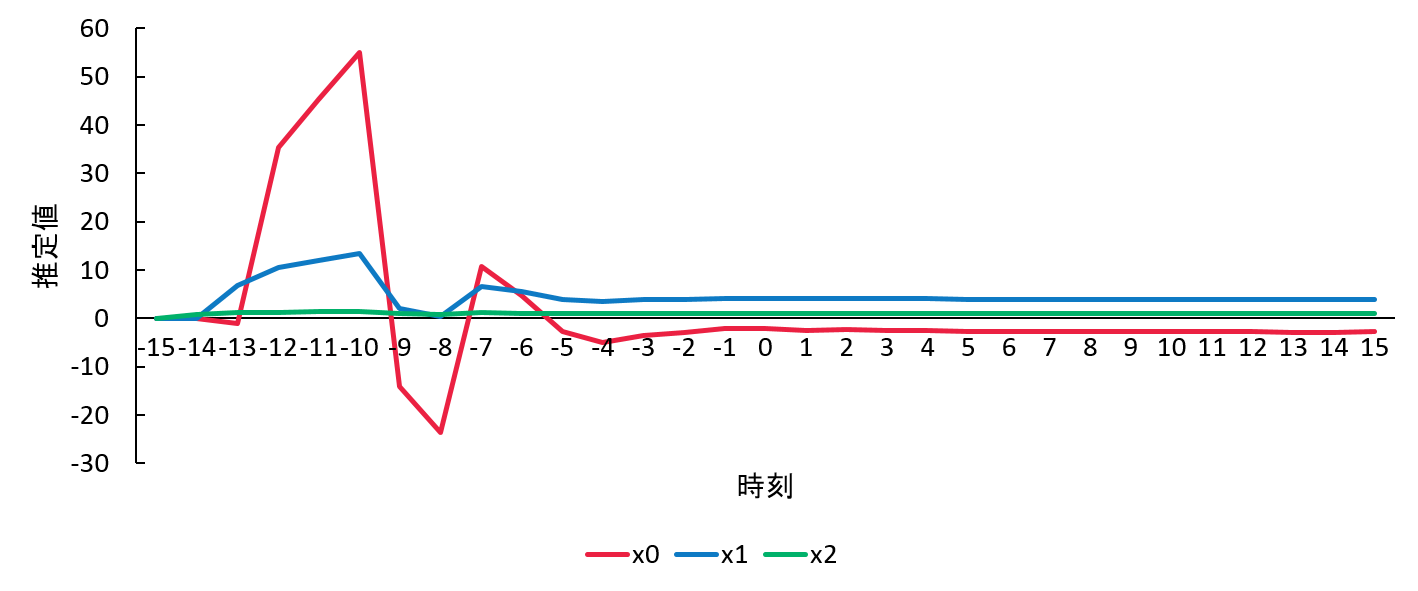
\includegraphics[width=16cm]{kalman1.png}
  \caption{カルマンフィルタによる推定値の時系列グラフ}
 \label{graph}
\end{figure}


リスト2より,時刻$a$が15のとき推定値は\(x_{0}=-2.804, x_1 = 3.977 x_2 = 1.001\)となっており,正しく推定できていることがわかる.また,図1より,推定値が収束していることがわかる.

%-----------------------------
%3章
%-----------------------------
\newpage
\section{カルマンフィルタにおける推定精度への影響}
\subsection{カルマンフィルタにおけるプラント雑音の共分散に対する推定精度への影響}

カルマンフィルタにおいて,プラント雑音の共分散に対する推定精度への影響を検証する.
ここで,サンプリング周期を$\tau$とするときプラント雑音の共分散は
\(
\mbox{\boldmath $Q$}_{(k)} =
\begin{bmatrix}
\frac{\tau^5}{20} & \frac{\tau^4}{8} & \frac{\tau^3}{6}\\
\frac{\tau^4}{8} & \frac{\tau^3}{3} & \frac{\tau^2}{2}\\
\frac{\tau^3}{6} & \frac{\tau^2}{2} & \tau \\ 
\end{bmatrix} q
\)
とする.また,初期推定誤差共分散は,
\(
\mbox{\boldmath $P$}_{(0)} =
\begin{bmatrix}
{10000} & 0 & 0\\
0 & {10000} & 0\\
0 & 0 & {10000} \\ 
\end{bmatrix} 
\)
とする.

\(\tau=0, 10^{-6}, 10^{-3}, 10^{0}, 10^{3}, 10^{6}\)の6つの場合における,カルマンフィルタによる推定値の時系列グラフを図2に示す.

\vspace{0mm}
\begin{figure}[!h]
  \centering
  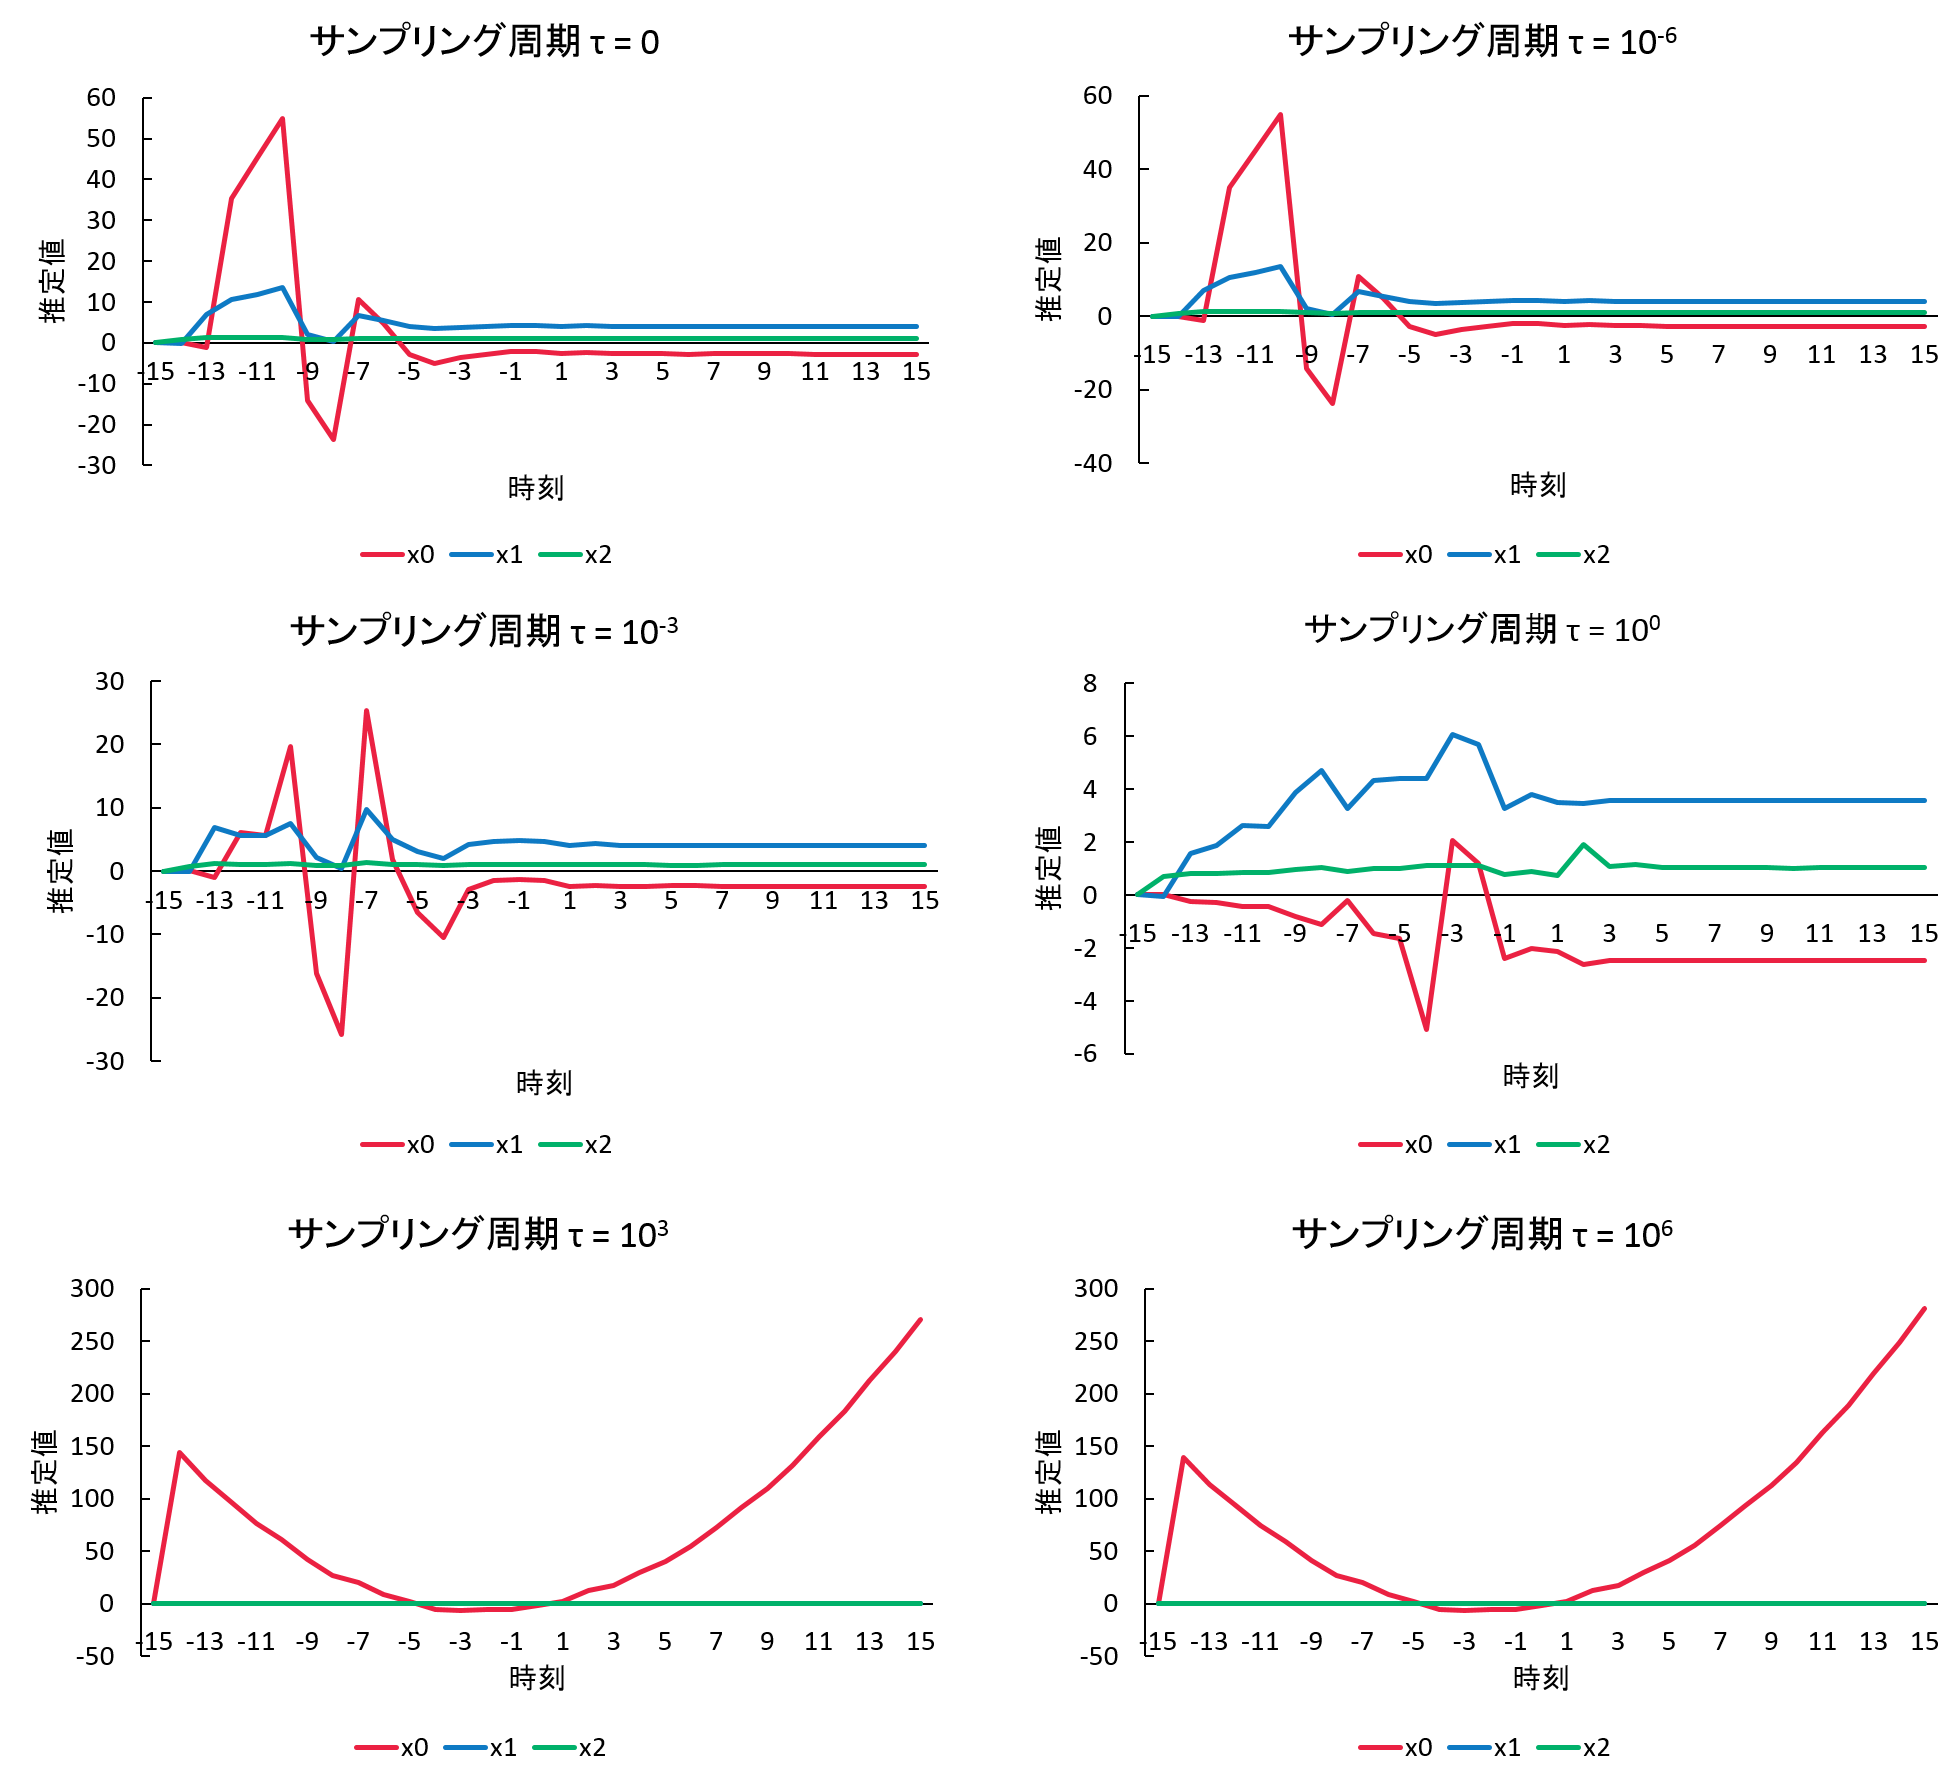
\includegraphics[width=14cm]{kalman2.png}
  \caption{サンプリング周期$\tau$を変化させた際の推定値の時系列グラフ}
 \label{graph}
\end{figure}


図2より,サンプリング周期$\tau$の値を0から徐々に大きくすると,推定値の誤差の振れ幅は小さくなるものの,収束までにかかる時間が長くなることがわかる.
また,サンプリング周期$\tau$が大きくなりすぎると推定値が発散してしまい,推定できないことがわかった.

\subsection{カルマンフィルタにおける推定値の初期共分散に対する推定精度への影響}
カルマンフィルタにおいて,推定値の初期共分散に対する推定精度への影響を検証する.
このとき推定の初期共分散は,
\(
\mbox{\boldmath $P$}_{(0)} =
\begin{bmatrix}
{p} & 0 & 0\\
 0 & {p} & 0\\
0 & 0 & {p} \\ 
\end{bmatrix} 
\)
とする.
また,サンプリング周期は$\tau = 10^0$とする.

\(p=0, 10^{-6}, 10^{-3}, 10^{0}, 10^{3}, 10^{6}\)の6つの場合における,カルマンフィルタによる推定値の時系列グラフを図3に示す.

\vspace{0mm}
\begin{figure}[!h]
  \centering
  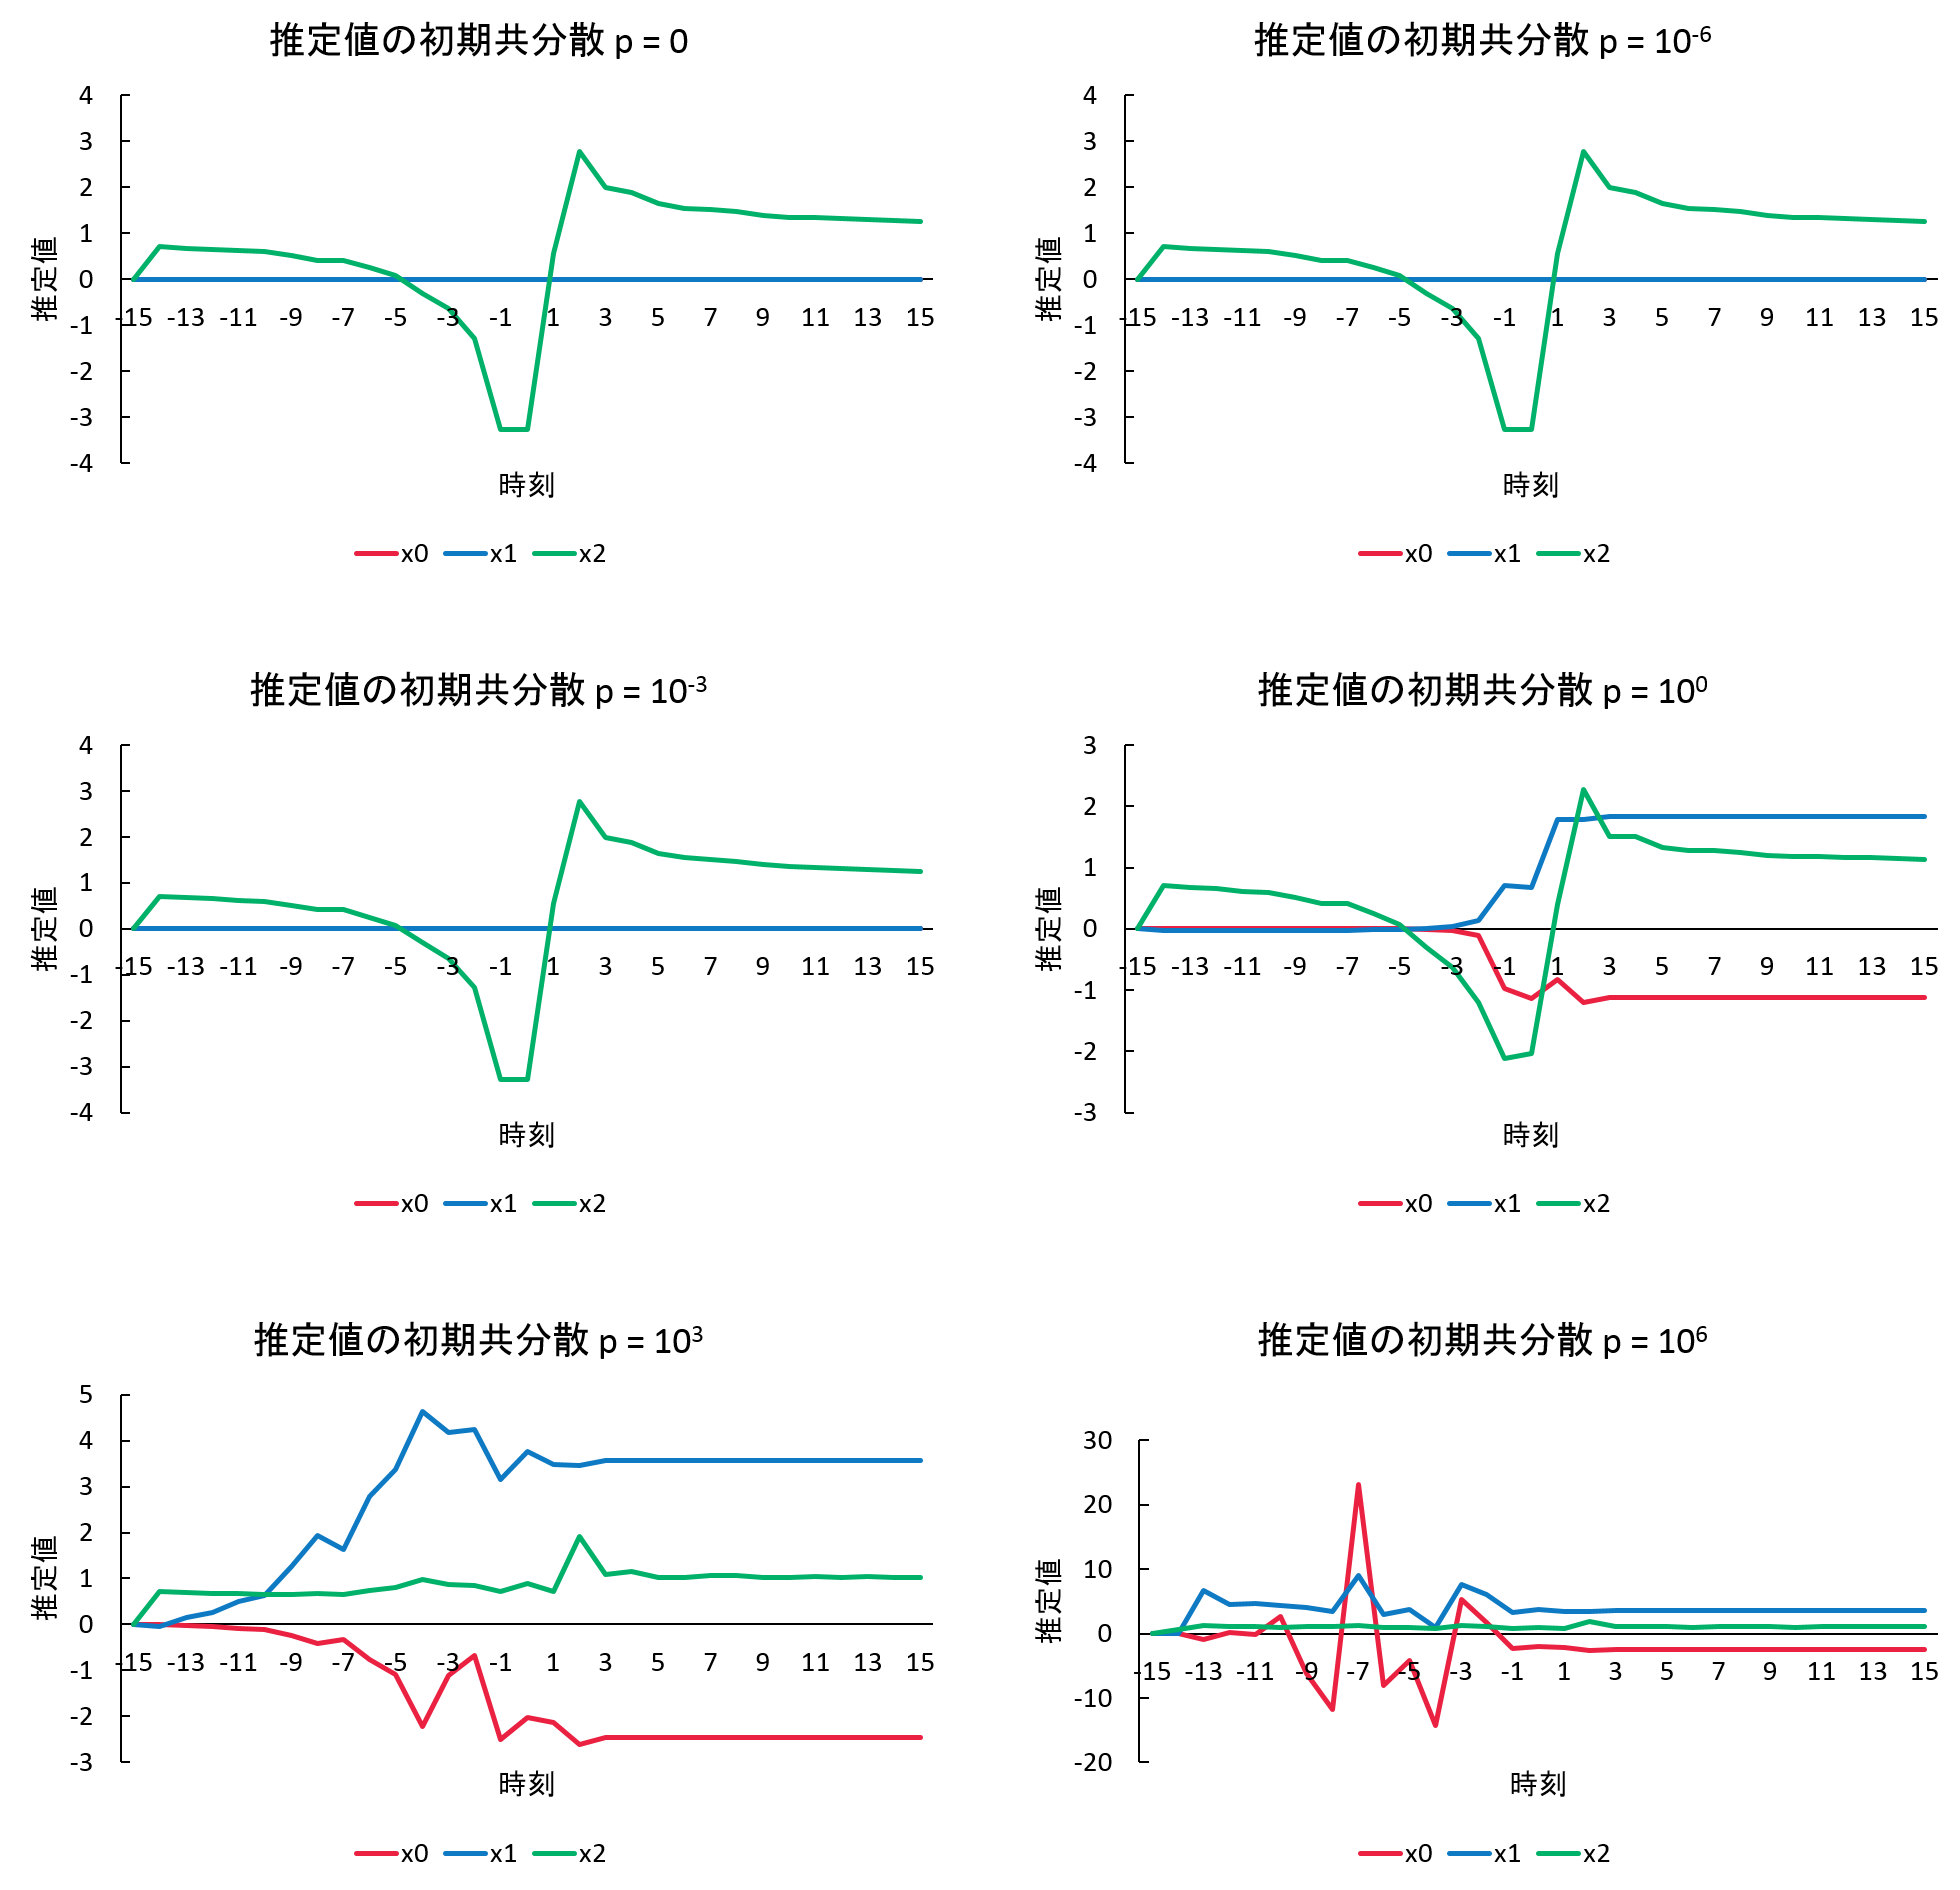
\includegraphics[width=14cm]{kalman3.png}
  \caption{推定値の初期共分散$p$を変化させた際の推定値の時系列グラフ}
 \label{graph}
\end{figure}


図3より,サンプリング周期$\tau = 10^0$の場合初期推定誤差共分散の値が小さすぎると,推定値$x_0,x_1,x_2$の値がおおよそ同じ値となり,時系列グラフの形状が変化しないことがわかった.
一方,初期推定誤差共分散の値が大きなると,収束するので推定が可能であることがわかる.
これより,初期推定誤差共分散を非常に大きくすることで推定誤差が小さくなることがわかる.
これは,推定誤差共分散が小さいということはその値が真値に近いことを示しているためあまり補正されないが,推定誤差共分散が大きいと真値から離れていることを示すので大きく補正がされることが原因であると考えられる.

\end{document}